\chapter{Mass and redshift estimation}\label{CH_03}

Fitting the spectral energy distributions (SEDs) of galaxies is an almost universally used technique to derive a range of physical properties of galaxies, such as redshift, stellar masses, star formation rates, dust masses, and metallicities (though there is a temptation to over-interpret the available data, so results should be taken with caution). SED fitting has matured significantly in the last decade and model predictions and fitting procedures have increased the precision of the results, attempting to keep up with the vastly increased volume and quality of available data. For this project we will use SED fitting to estimate redshift of individual galaxies and their corresponding stellar mass.

Traditionally, photometric redshift estimation is generally presented by two large groups of algorithms: empirical methods and the template-fitting methods (not to be confused with the template-fitting technique that we use to perform photometry on near-IR images). Empirical methods use a subsample of the photometric survey with spectroscopically-measured redshifts as a "training set" for the redshift estimators. This subsample describes the redshift distribution in magnitude and color space empirically and is used then for calibration of the whole sample. We list several training set based codes: ANNz \citep{2004PASP..116..345C}, RFPhotoZ \citep{2008ASPC..394..521C}, Singal \citep{2011PASP..123..615S}. Template methods use libraries of either observed spectra of galaxies exterior to the survey or template SEDs, that are built using different stellar population synthesis (SPS) models. As these spectra are produced artificially, they span over full spectra, and templates can be shifted to any redshift and then convolved with the transmission curves of the filters used in the photometric survey to create the template set for the redshift estimators. Among some most widely used template based codes we list BPZ \citep{2011ascl.soft08011B}, HYPERZ \citep{Bolzonella2011} and Kcorrect \citep{Blanton2017}. Both methods then use these training sets as bases for the redshift estimating routines, which include $\chi^{2}$-fitting and various machine learning algorithms (e.g. artificial neural networks, ANNs). A good review of the present state of the art in the area of fitting SED of galaxies is presented in \citep{Walcher2011} and a list of codes with documentation, reviews, discussions and templates is available at \fnurl{sedfitting.org}{http://www.sedfitting.org/Fitting.html}

For several years best results in SED fitting were obtained by the codes that calculate redshift based on the flux determined from the red-sequence stars - redMaPPer \citep{2014ApJ...785..104R}, redMaGiC \citep{2015MNRAS.453...38R} or that use a trained neural network (ANNz \citep{2004PASP..116..345C}). Recent studies \citep{Bundy2015} show that these codes get twice smaller scatter of z\_phot vs z\_spec for massive galaxies. But for the faint galaxies (i-band magnitude $> 22.5$ AB), template codes perform slightly better, probably because of the smaller training sets available for neural networks and obviously poorer photometry. Our catalog consists of over 23 millions of objects, and calculation speed is also an important factor for the section of the fitting code. Computationally, most template-fitting codes benchmark roughly similarly, while the training codes are much faster to evaluate the redshifts but only after their training is complete. The quality of our data was refining while the project was already ongoing and we did not attempt to use the empirical-based codes as it would have required re-computation of the training set after each change in the algorithm (e.g., we did not plan to perform matching to the u-band PSF originally). Thus we chose to test several template-fitting codes to find which one gives the best results.

\section{SED fitting}

\subsection{Choice of SED fitting codes}

A special case of analyzing SEDs of extragalactic sources
is the problem of redshift estimation, a topic that is usually
referred to as photometric redshifts (hereafter z\_phot). This
problem is different from all other estimates of physical properties (stellar mass, star-formation rate, mass of dust and gas, age) because independent and more precise measurements of the same property are available for large samples in the
form of spectroscopic redshifts (assuming some cosmological model). Results of SED fitting can thus be
tested extensively and parameters are calibrated empirically. It is also
historically one of the earliest forms of SED fitting, having been suggested as a manner to go beyond the limits of early spectroscopy \citep{1957AJ.....62....6B}.

We performed our own analysis using the first set of data that we got in the SHELA region \citep{Papovich2016}. It covers $\approx24$ $deg^{2}$ and contains over 1,800,000 sources. We do cross-matching between our catalog and SDSS DR14 release using SQL Query CasJobs. The table "SpecObj" contains data from all available SDSS spectroscopic catalogs. There are 15,790 sources in our catalog that have counterparts in SDSS DR14 within 1" and have spectroscopic redshift. We used this sample to test photometric redshifts produced by three different SED fitting codes - HYPERZ \citep{Bolzonella2011}, LePhare \citep{Arnouts2011} and EAZY \citep{Brammer2008}.

HyperZ and LePhare produced marginally the same results with the only difference that LePhare does not assign a source with the photometric redshift if the $\chi^{2}$ value is too high. Our research suggests using information from as many sources as possible and we turned down LePhare.

Tests of EAZY reveal not just the tighter correlation between spectroscopic and photometric redshifts, but also significantly smaller CPU time needed. EAZY works approximately 10 times faster and computes redshifts for a catalog that contains 50 thousands sources in 10 minutes. Considering the size of our catalog, EAZY was a natural choice for the photometric redshift determination.

We observe an unusual scatter in our data around redshift $z\approx0.4$ when comparing to the spectroscopic sample. Similar behavior can be seen in See Figure 4 in Bundy 2015 \citep{Bundy2015}, Figure 7 in Rowan-Robinson \citep{Rowan-Robinson2008} and Figure 11 in Brammer et al. \citep{Brammer2008}. SED fitting technique depends on strong features in the SEDs of the objects, such as the Balmer break, strong emission lines or even PAH features \citep{2009MNRAS.394..375N}. We try to investigate the nature of such scatter. It may not be due to the misidentification of the Lyman break as the Balmer/4000A break because we have very few galaxies with $z>1$ in our sample. Next, we examine the possibility that strong emission lines can alter the redshift. We downloaded SDSS DR14 data for certain emission lines and used flux and emission width of O[II], O[III] and Halpha lines. We compared two sets of galaxies around z=0.4 - the one with correct identification of the photometric redshift and the other that has severe offset. We did not observe any correlation between deviation of the photometric redshift from spectroscopic one and the strength of any lines.

This scatter can be slightly reduced by rejection of certain templates available for SED fitting, but there is not strict justification for choice of any particular template that is rejected, so we did not proceed in this way. We claim that such scatter in redshift determination should not affect our main results and we address this issue in the next chapter (binning).

\subsection{EAZY and FAST}

We used EAZY code to compute photometric redshifts based on optical and near-IR fluxes that we accumulated in our catalogs. EAZY \citep{Brammer2008} is photometric redshift code which was written for samples with incomplete and/or biased spectroscopic information. The code combines features from various existing programs: the possibility of fitting linear  combinations of templates (as done in GREGZ), the use of priors (as first done in BPZ), and a user-friendly interface based on HYPERZ. The default template set and the redshift-magnitude priors are derived from semi-analytic models. These models are, of course, only an approximation of reality, but their full completeness down to very faint magnitudes outweighs their imperfect representation of the real Universe. 
Calculation of the photometric redshifts is made based on the linear combination of templates. We used the latest available set of templates (v1.3) provided by Brummer on \fnurl{GitHub}{https://github.com/gbrammer/eazy-photoz/blob/master/templates/eazy_v1.3.spectra.param}. These templates take into account presence of emission lines (Ha, Hb, OIII, OII, and Ly-alpha) in the following way: SFR  is estimated from the template "luminosity" at 2800 A and then Kennicutt-Schmidt (KS) {\citep{Schmidt1959}}, {\citep{Kennicutt1998b}} relations are used to add emission lines with fixed line ratios. Another template in this set is an evolved Maraston 2005 SSP, added because it was found that the reddest EAZY template didn't quite get red enough for massive old galaxies at $z<1$. Two last templates add old and dusty template (Brammer, in prep, 2014) and blue, high equivalent width line template based on \citep{2010ApJ...719.1168E} for low-z galaxies.

Run of the whole set of objects on cluster with EAZY takes less than four hours, so we were able to perform it multiple times, tuning parameters for the better estimation of the z\_phot. There are several output redshift estimates that one can use.
We took $z\_{m1}$ as our photometric redshift,  it is the redshift marginalized over probability distribution $p(z\mid C)$, where z is a redshift and C - color of the source

Results are compared against available SDSS DR14 spectroscopic data. On Figure~\ref{fig:photo_z} we plotted the our results in two different fashions: z\_phot vs z\_spec (top) and a difference between those two results against z\_spec (bottom).

\begin{figure}[!ht]
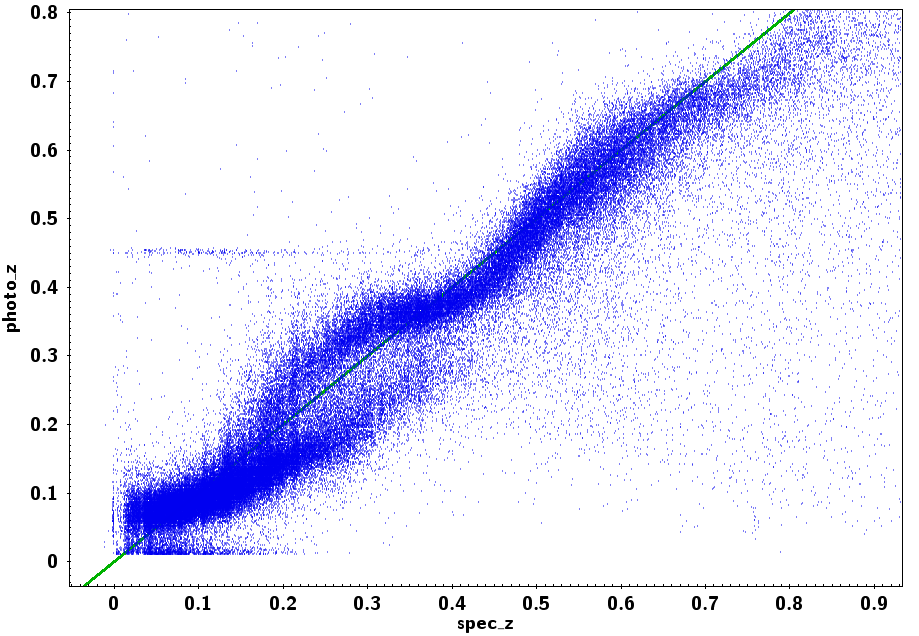
\includegraphics[width=5.7in]{Figures/photo_z_vs_spec_z.png}
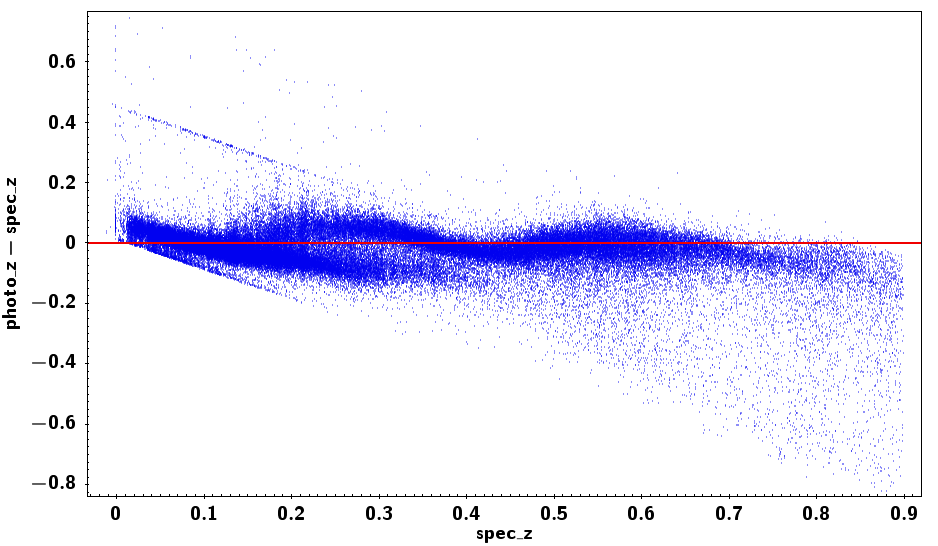
\includegraphics[width=5.7in]{Figures/photo_z_-_spec_z.png}
\caption{Comparison of z\_phot as calculated in EAZY to the z\_spec from the SDSS spectroscopic data. z\_phot vs z\_spec is plotted on top, another version of this plot, z\_phot - z\_spec vs z\_spec is plotted at the bottom. Despite several observable issues (especially around $z\approx 0.4$) the overall fit is satisfactory with the standard deviation as low as $\sigma=0.07$.}
\label{fig:photo_z}
\end{figure}

We provide the full list of EAZY parameters in \hyperref[sec:eazy]{Appendix}.

\subsection{Reliability of IR data}
It is well known that template errors in the rest-frame
near-IR can lead to degraded photo-z performance when
near-IR data is included (e.g., \citep{Brammer2008}).
\citep{2012AJ....144..188B} demonstrated acceptable z\_phot
performance with near-IR magnitudes included. They confirm that
the addition of UKIDSS photometry here does not improve the template z\_phot results, but also does not degrade them if photometry is appropriately weighted to
take template errors into account. 

We perform another run of EAZY with only optical photometry provided as input and compare the standard deviation of z\_spec vs z\_phot. As can be seen in Figure~\ref{fig:photo_z_nowise} near-IR filters do not significantly change the accuracy of the redshift estimation.

\begin{figure}[!ht]
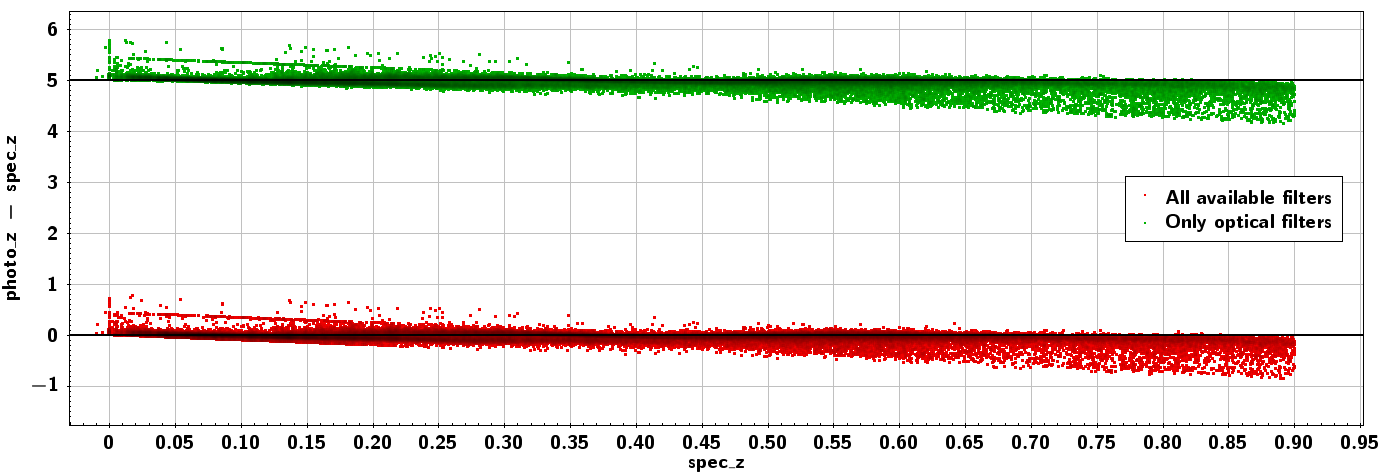
\includegraphics[width=5.7in]{Figures/photo_z_-_spec_z_nowise_wise.png}
\caption{Difference of z\_phot and z\_spec is plotted against z\_spec. Data obtained with all 7 or just 5 optical filters are plotted in red and green respectively.}
\label{fig:photo_z_nowise}
\end{figure}

\subsection{Stellar masses}

FAST (Fitting and Assessment of Synthetic Templates) \citep{2018ascl.soft03008K} is originally an IDL-based code that fits stellar population synthesis (SPS) \citep{2003MNRAS.344.1000B} templates to broadband photometry and (or) spectra. FAST is compatible with EAZY when fitting broadband photometry - it uses the photometric redshifts derived by that code as an input redshift. 
IDL (Interactive Data Language), is a programming language used for data analysis, it requires a license and is not installed on MU cluster machines so instead we use FAST++, a C++ version of FAST that can be found at \fnurl{GitHub}{https://github.com/cschreib/fastpp}. FAST++ code uses same input and output formats as FAST, is at least 4 times faster and apart from the single-threaded FAST is multithreading - it may use a number of concurrent threads (CPUs) that the program can use to speed up calculations, which is a significant advantage when working with a data sample as large as ours.
We tried several combinations of codes such as:\\
HyperZ for redshift estimation and FAST for stellar mass estimation;\\
HyperZ for redshift and stellar mass estimation;\\
EAZY for redshift estimation and HyperZ for mass estimation;\\
EAZY for redshift estimation and FAST for mass estimation;\\
and found the last option to be working best. So after we got photometric redshifts for all sources in our catalog with $SNR>5$ and non-zero flux in more than 4 filters, we supplied it along with the flux in $\mu$Jy to the FAST code. It takes around 12 hours CPU time to calculate masses for a set of $\approx60,000$ sources, so we used Lewis computational cluster again.
We present the mass histogram for four redshift bins of equal size on Figure~\ref{fig:hist_mass}. We see that galaxies in the lowest redshift bin are on average less massive then and tend to have stellar mass of $\sim10^{8.8}M_{sun}$, while galaxies in the higher redshifts peak around mass of $10^{10}M_{sun}$. This is can be explained by the incompleteness of our sample in high redshifts.

\begin{figure}[!ht]
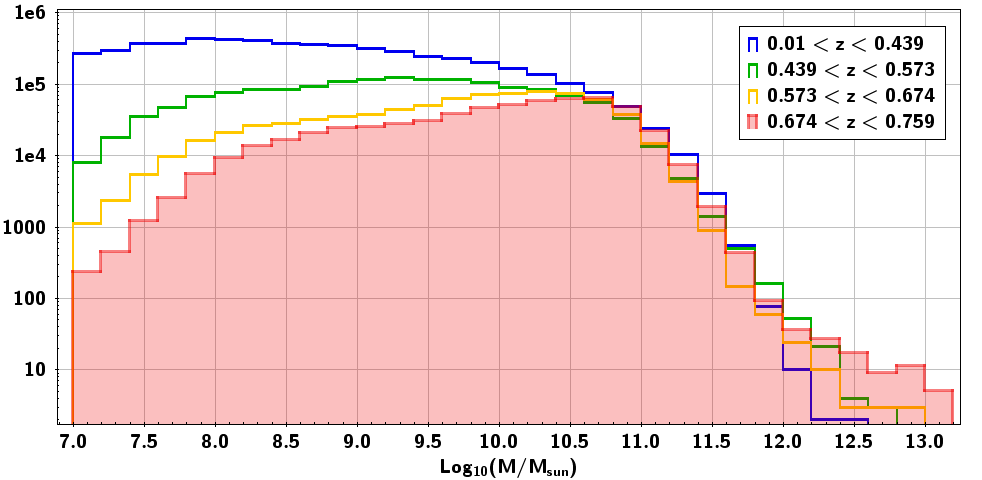
\includegraphics[width=5.7in]{Figures/histogram_all_stellar_mass_z_bins.png}
\caption{A histogram of masses for all four redshift bins. Galaxies in different bins end to peak at different masses, but galaxies in three high-redshift bins have the highest number of galaxies around similar stellar mass - $10^{10}$}
\label{fig:hist_mass}
\end{figure}

\section{Catalog post-procession}

At this point every source that has photometry in more than 4 filters has z\_phot and stellar mass assigned to it. But this data sample is not clean - there are stars, QSOs, also there are duplicate sources and sources with unreliable near-IR photometry due to the presence of nearby saturated sources. In the following subsections we explain our strategy of constructing the clean sample of galaxies.

\subsection{Star-galaxy separation}

Performing the classification of the sources is an important step in our project. Indeed, SED fitting codes may take photometric data of the star as a valid input and assign it some photometric redshift and stellar mass that does not have any physical significance ($\chi^{2}$ value of such objects is usually low, but this criteria is not enough to rejects stars). Such objects may severely alter the global density of objects and skew our results. In this section we attempt to find select galaxies alone from our sample and reject stars and other sources (mainly QSO) that are not a part of this project. Such selection is usually referred to as a "star-galaxy separation". One of the standard ways of performing this separation is via color-color diagram, on which stars and galaxies (hopefully) occupy different space on the graph. We tested several combination of bands in order to achieve best results (i.e. maximum possible number of galaxies rejected and minimal number of non-galaxies included in the sample) and found out that $"w1-i\; vs\; i-z"$ colors works best. As can be seen on (Figure~\ref{fig:sgs_color}), galaxies (blue), stars (red) and QSO (green) indeed occupy different space but with large overlapping regions, so the data set will neither be clean, nor complete. Another complication is that while we used r-band as a detection for the optical catalog and so all optical sources have consistent photometry in all 5 bands, some sources are shallow or undetected in w1 band. Such sources are assigned with w1\_{mag}=99 and thus occupy a low-left part of this diagram, outside of the reasonable regions. 

\begin{figure}[!ht]
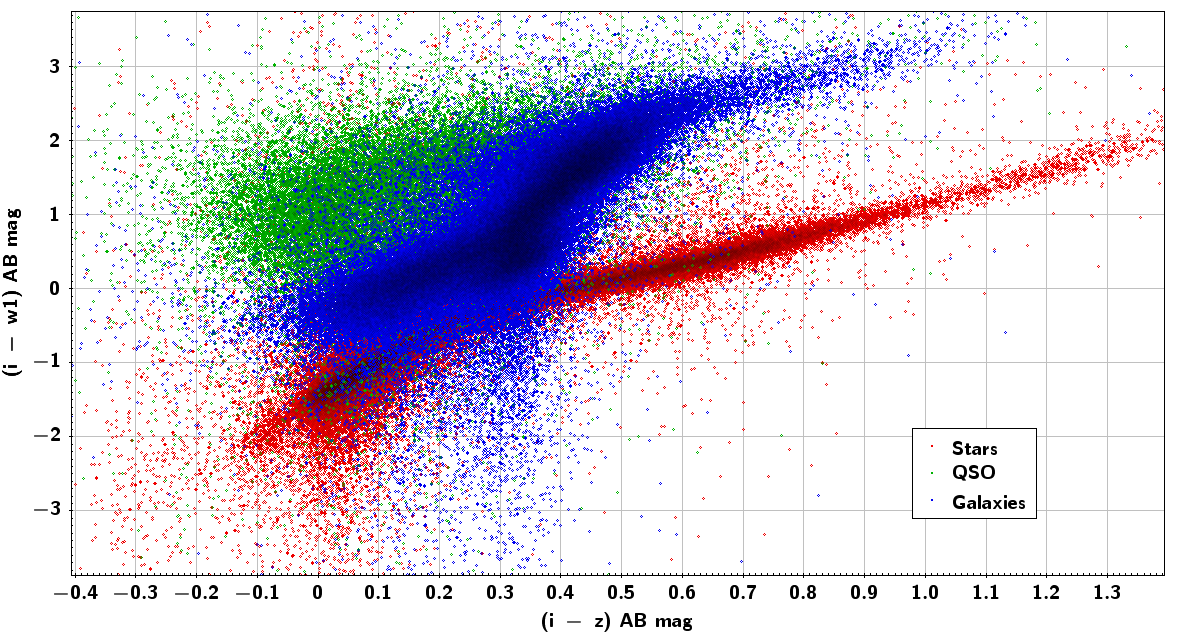
\includegraphics[width=5.7in]{Figures/star_galaxy_separation_color.png}
\caption{Color-color diagram for star-galaxy separation using $"w1-i\; vs\; i-z"$ colors.  Galaxies are plotted in blue, stars - in red and QSO in green. It is impossible to create a clean data sample using only colors as a selection criteria.}
\label{fig:sgs_color}
\end{figure}

Lack of IR data for some objects is a real disadvantage of the star-galaxy separation based on the color-color diagram, so we shall use another approach that is based on the "CLASS\_STAR" value - a stellarity index given by {\tt SExtractor}. Stellarity values near "0" indicate the object is likely a galaxy. If stellarity values near "1" that is a good indicator that an object is likely a star. To classify objects, {\tt SExtractor} uses a neural network which takes into account object attributes including FWHM. 
So the outline of our algorithm is as follows: the PSF functions that we built for every SDSS image will be used to measure FWHM of this image using {\tt irif/psfmeasure} task. Then this FWHM shall be supplied to the parameter file of SExtractor and another run of this code is performed in g-, r-, and i-bands (these bands are the most sensitive and generally have better FWHM over u- and z-bands).

Star-galaxy classification based on the CLASS\_STAR parameter that is measured in one band is about 95\% accurate (Figure~\ref{fig:sgs_hist}). We attempt to refine this result by finding the combination of selection criteria in three bands instead of just one.
We downloaded SDSS DR14 BOSS and SDSS spectrograph data in Stripe 82 region using \fnurl{CasJob Server}{https://skyserver.sdss.org/CasJobs/}. The size of this data set is 269,196 sources, each of which is assigned with spectroscopic class (can be GALAXY, QSO, or STAR) and extragalactic objects galaxies and QSO are also assigned with the z\_spec larger than 0. By matching this catalog to our main output catalog we got a set of data that contains 248,682 sources, which will serve as a training set for our star-galaxy separation.
We found the next criteria to perform the bet way:
$CLASS\_STAR\_r<0.2 \quad \&\& \quad CLASS\_STAR\_g<0.34 \quad \&\& \quad CLASS\_STAR\_i<0.70$\\
\begin{figure}[!ht]
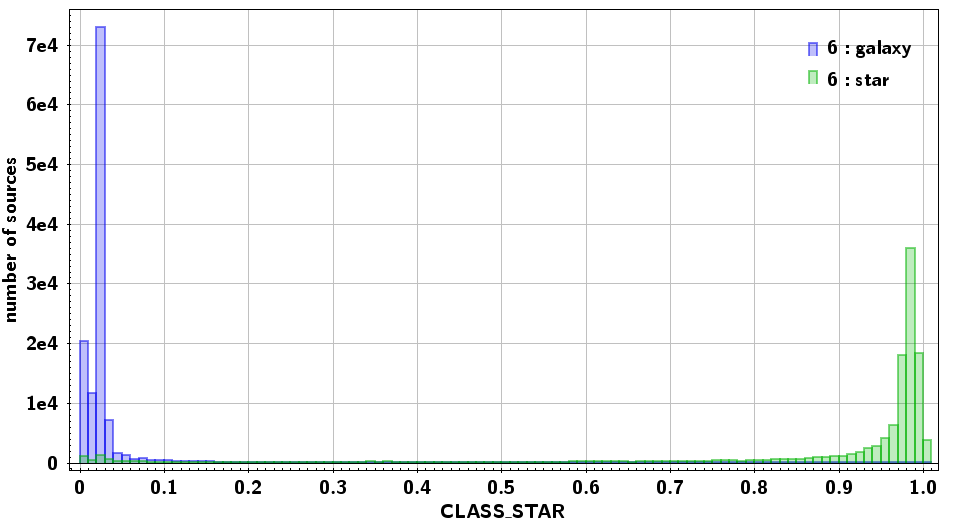
\includegraphics[width=5.7in]{Figures/histogram_class_star.png}
\caption{A histogram of the CLASS\_STAR values for r-band alone already shows efficiency of this method for star-galaxy separation. Galaxies and stars are selected from BOSS spectroscopic survey using parameter "CLASS". Galaxies are plotted in blue and tend to have smaller values of CLASS\_STAR, stars are plotted in green and on opposite - mostly have CLASS\_STAR value close to 1.}
\label{fig:sgs_hist}
\end{figure}

After this criteria has been applied to the data set we found that 3,874 galaxies (1.55\%) fall outside of the catalog and 4298 (1.73\%) stars and QSO are included into the sample (Figure~\ref{fig:sgs_hist}). We are satisfied with this result and perform the above criteria to the whole data set that decreases our total number of sources from 26,585,975 to 10,092,410 objects.

\begin{figure}[!ht]
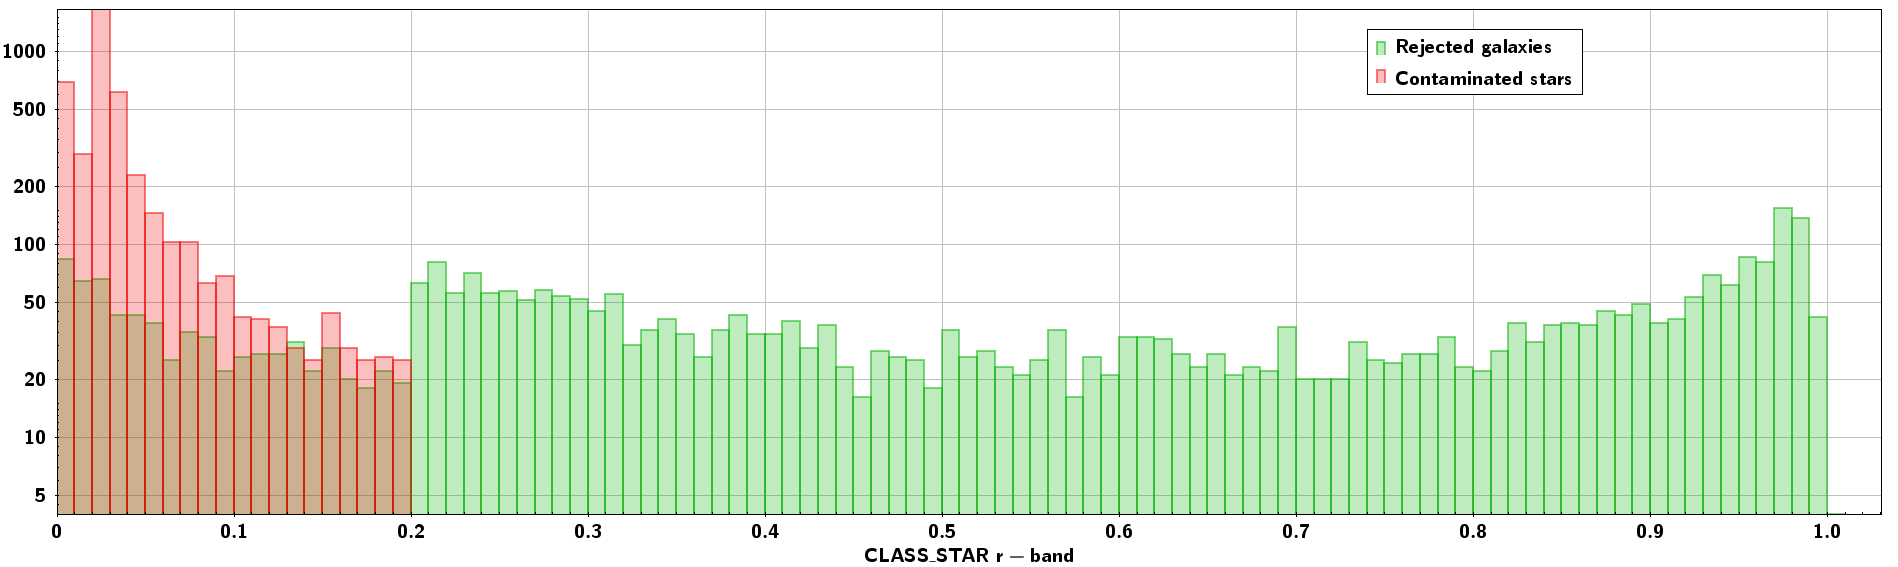
\includegraphics[width=5.7in]{Figures/histogram_class_star_contamination.png}
\caption{A histogram of the CLASS\_STAR values for galaxies from the control data sample that are rejected from our data sample due to very large CLASS\_STAR values (green). In red we plotted stars and QSO that are not excluded from our data sample - their CLASS\_STAR values are too small in all three optical bands that we used for star-galaxy separation.}
\label{fig:sgs_cont}
\end{figure}


\subsection{Sources treatment in overlapping regions and around bright stars}

Two adjacent SDSS images have overlapping regions - 25" wide for images in the same columns (i.e. their centers have the same Dec) and 28" wide for images in the neighbor columns (i.e. their centers have the same RA). Sources that appear in such regions are {\tt SExtracted} and {\tt TPHOTed} twice and have to be removed from the final catalog. We perform internal match on the catalog within all 80 unWISE frames and remove duplicate sources within 1.2 asec matching radius using {\tt STILTS} code. We verify that this radius is sufficient for removing majority of duplicate sources and also does not remove any non-duplicate sources in the main field that may have similar coordinates. This operation reduced the number of galaxies in our sample to 9,308,387 sources. An example of such duplicate sources is plotted with blue on Figure~\ref{fig:duplicate}

\begin{figure}[!ht]
\center{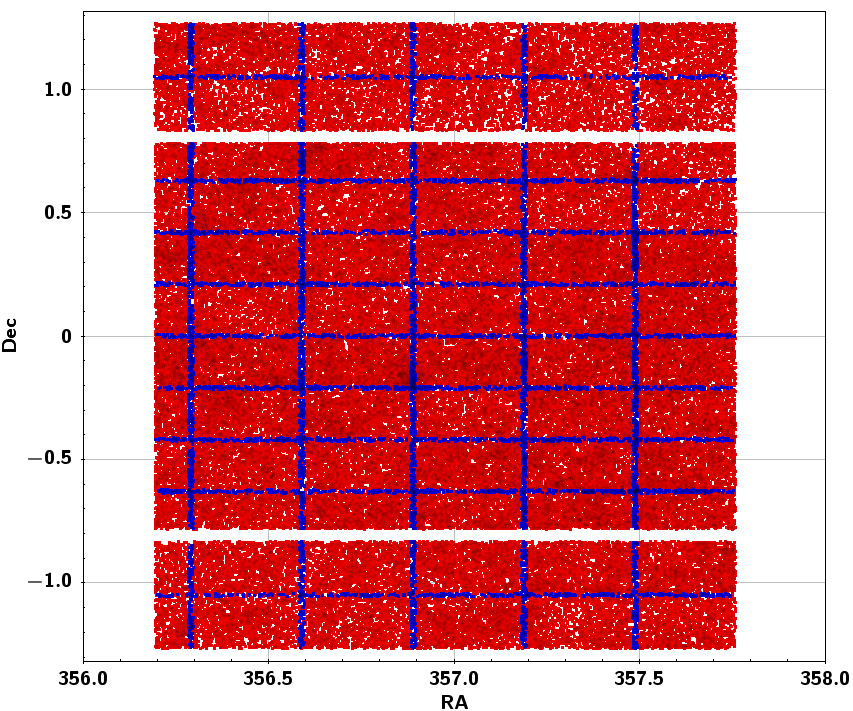
\includegraphics[height=4in]{Figures/duplicate_sources.png}}
\center{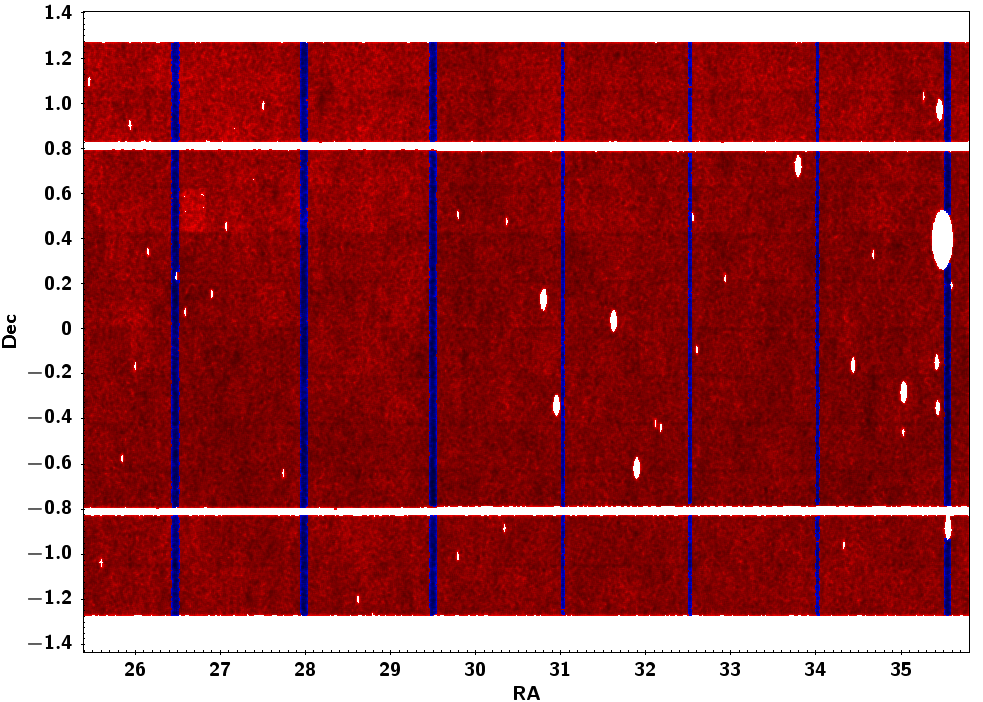
\includegraphics[height=4in]{Figures/duplicate_sources_wise.png}}
\caption{Duplicate sources (blue) are over-plotted with unique sources (red) in one unWISE frame that hosts 72 SDSS images (top image) and several adjacent unWISE frames (bottom image). Two white horizontal stripes between col07 and col02 (bottom) and coll11 and col06 (top) were also excluded from our project.}
\label{fig:duplicate}
\end{figure}

One unWISE frame consists of 3 unWISE images that have the same RA and are centered at Dec=$-1.6^{0}$, $0.0^{0}$ and $+1.5^{0}$. When we plotted SDSS images over unWISE frame, we noticed that each SDSS image from col07 and unWISE file that is centered at Dec=$+1.5^{0}$ overlap in a small region $\approx52.28$ square minutes. To process this small area in {\tt TPHOT} another 2,315 PSFs have to be constructed. We decided not to perform this very time-consuming operation and exclude this area, in total 5.55 $deg^{2}$ from our project. The same situation is with SDSS images from col02 and unWISE files centered at Dec=$-1.6^{0}$. Total area that was excluded from the project is 11.340 $deg^{2}$, it may be sen as two white horizontal stripes on Figure~\ref{fig:duplicate}

Objects that are extremely bright in near-IR present a number of problems to the photometry measurement by generating a host of artifacts. These artifacts include halos (low surface brightness emission extending well beyond the PSF), diffraction spikes, horizontal stripes and residual ghosts.
If not corrected, these artifacts will compromise the reliability of w1 and w2 photometry performed by TPHOT. To account for such artifacts the natural solution is to mask certain regions based on available catalogs. We used SAO star catalog \citep{Staff1966} and Bright IR Stars Compilation (BIRSC) [R. Tam and C. Xu - IPAC] as a base for the masking catalog. There are around 400 stars in both catalogs that fall within Stripe 82 footprint, but our visual inspection showed that some very bright objects (stars and galaxies) that severely alters results of {\tt TPHOT} are not in this list. We inspected all residual FITS images and added 300 more objects to the list that now consists of 706 objects. For stars from the catalog the masking area depends on the provided V-band magnitude and it was assigned manually based on the estimation of the halo for the added objects. Radii for masking are ranging from 50 to 500 arcsec. An example of such source with masking radius=100 asec is presented on Figure~\ref{fig:masking}. The overall masked area is 3.871 $deg^{2}$, which reduces the total sky area of the survey to 288.212 $deg^{2}$.

\begin{figure}[!ht]
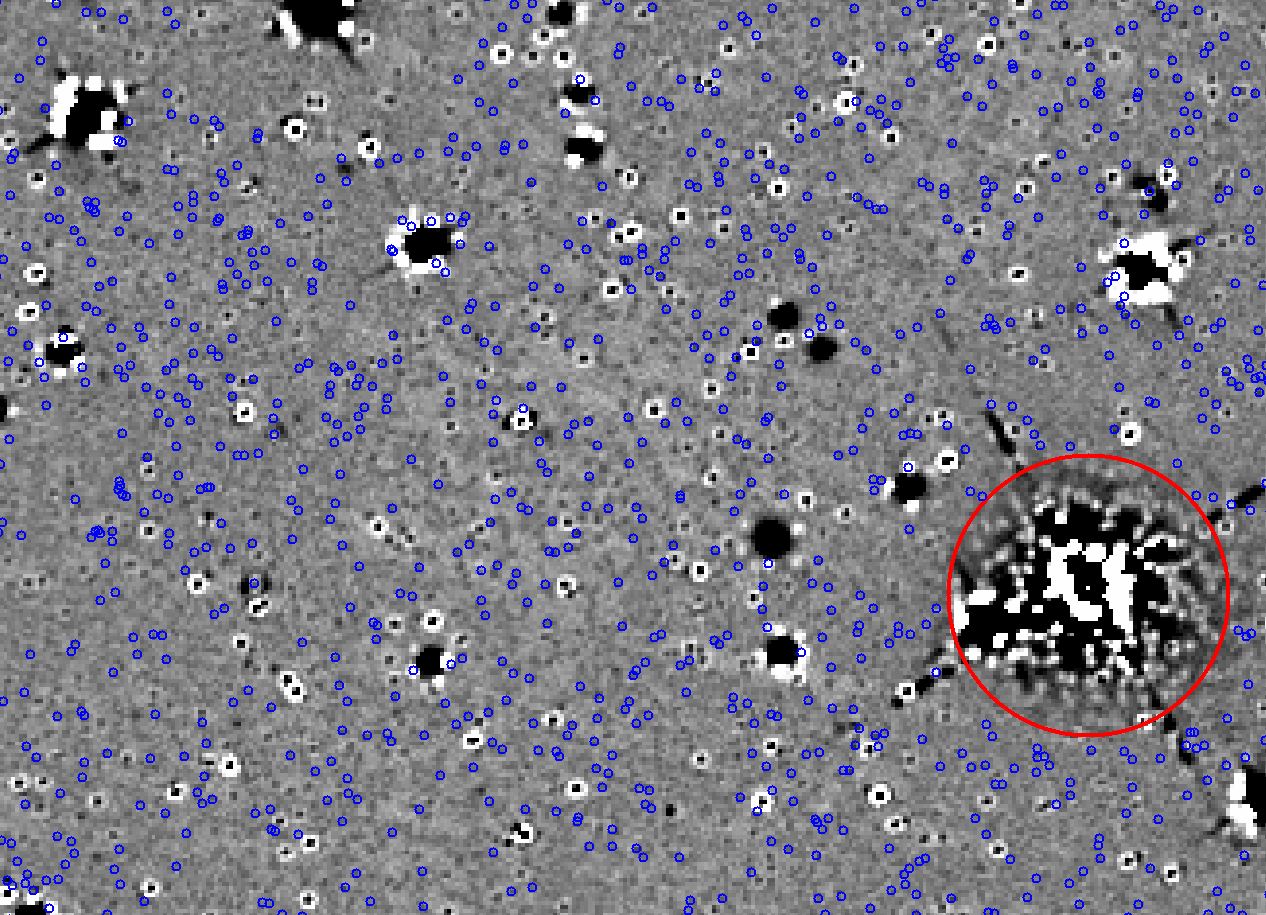
\includegraphics[width=5.7in]{Figures/CS_fits_region.png}
\caption{Residual image in w1 band with various regions plotted. All sources that were detected in r-band and supplied to TPHOT, but fall within the masked region (red) are excluded from the SED fitting. Blue circles 3 asec in radius show the position of objects, whose flux was subtracted from the unWISE image. Poorly subtracted objects (mostly stars) without blue circles around them were included into TPHOT input catalog, but later were excluded from ED fitting after star-galaxy separation}
\label{fig:masking}
\end{figure}

After rejection of such objects our catalog contains 9,061,068 objects and this is the final sample that we use as input to SED fitting codes that return photo$\_z$ and stellar mass that we use to build GSMD.